\documentclass[tikz,border=10pt]{standalone}
\usepackage{tikz}
\usetikzlibrary{calc}
\begin{document}
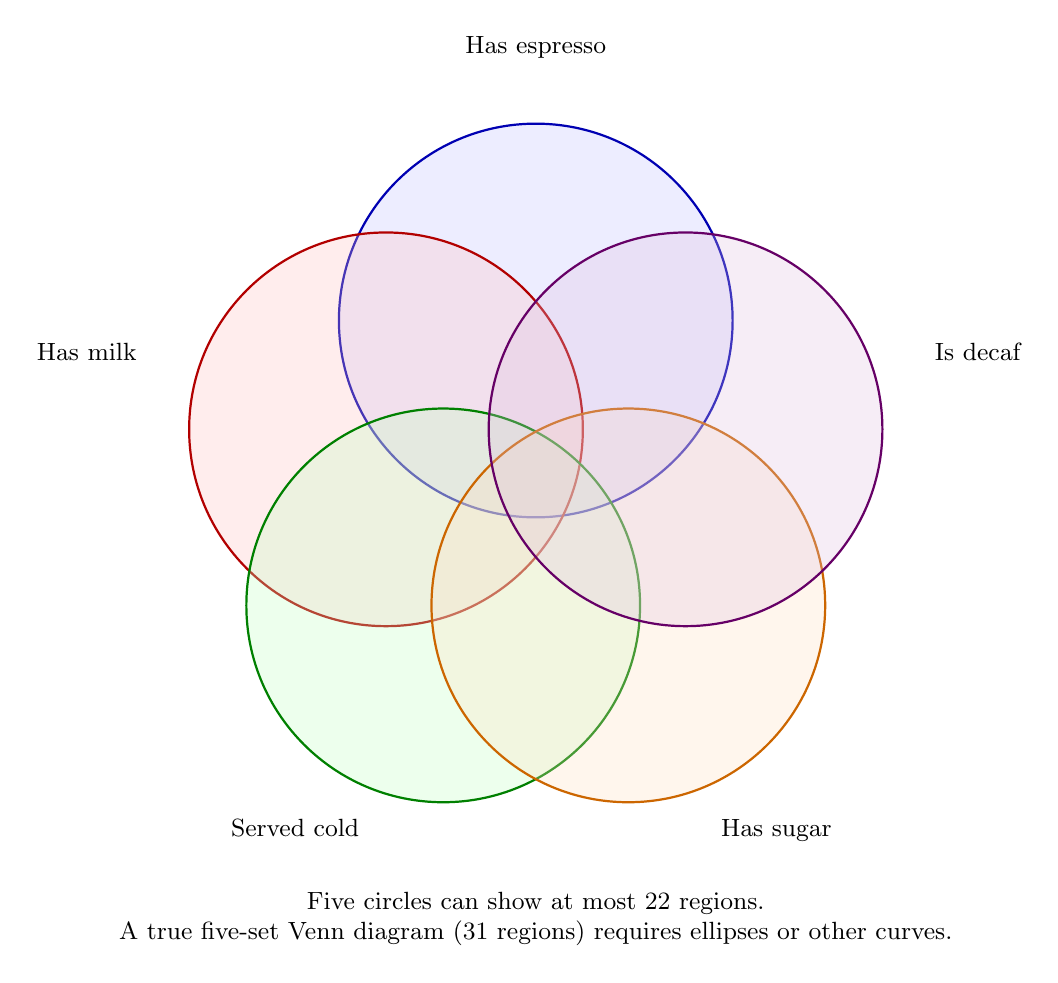
\begin{tikzpicture}[scale=1.0]
  % Five congruent circles centred on a regular pentagon.
  % All pairs overlap.  Five circles can form at most 22 regions;
  % a true five-set Venn diagram (31 regions) is impossible with circles.
  \def\R{2.0}
  \def\rad{2.5}
  \foreach \i in {0,...,4} {
    \pgfmathsetmacro{\ang}{90 + \i*72}
    \pgfmathsetmacro{\cx}{\R*cos(\ang)}
    \pgfmathsetmacro{\cy}{\R*sin(\ang)}
    % choose a colour and label
    \ifcase\i
      \def\col{blue!70!black}\def\fillcol{blue!25}\def\lab{Has espresso}
    \or
      \def\col{red!70!black}\def\fillcol{red!25}\def\lab{Has milk}
    \or
      \def\col{green!50!black}\def\fillcol{green!25}\def\lab{Served cold}
    \or
      \def\col{orange!80!black}\def\fillcol{orange!25}\def\lab{Has sugar}
    \or
      \def\col{violet!80!black}\def\fillcol{violet!25}\def\lab{Is decaf}
    \fi
    \draw[thick, draw=\col, fill=\fillcol, fill opacity=0.28]
      (\cx,\cy) circle (\rad);
    \pgfmathsetmacro{\lx}{(\R+\rad+0.7)*cos(\ang)}
    \pgfmathsetmacro{\ly}{(\R+\rad+0.7)*sin(\ang)}
    % anchor the label so it sits outside the circle
    \ifnum\i=0 \def\anc{south}\fi
    \ifnum\i=1 \def\anc{east}\fi
    \ifnum\i=2 \def\anc{north}\fi
    \ifnum\i=3 \def\anc{north}\fi
    \ifnum\i=4 \def\anc{west}\fi
    \node[font=\small, anchor=\anc, align=center] at (\lx,\ly) {\lab};
  }
  \node[font=\small, align=center] at (0,-5.6)
    {Five circles can show at most 22 regions.\\
     A true five-set Venn diagram (31 regions) requires ellipses or other curves.};
\end{tikzpicture}
\end{document}
